\documentclass[twoside,noframe]{ncuthesisXe}
\usepackage{makeidx}             % for index
\usepackage{layout}              % to show page dimensions
% 以下為中大碩博士論文封面 它校需自行更改ncuthesis.cls檔

\dept      {機械工程研究所}
\degree    {碩/博士}
\title     {模版 {\sf ncuthesisXe} 使用說明}
\subtitle  {\sf An example in \LaTeX/\XeLaTeX}

\author    {羅吉昌}
\mprof     {羅吉昌}
\sprof     {共同指導:甲教授\\ \hspace{2.3cm} 乙教授} 
\degreedate{中~華~民~國~一百零一~年~六~月}
\copyyear  {2012}

% \newcommand\insertfig[2]{
\begin{figure}[!hbt]
\centering
\includegraphics[scale=2]{#1}
\caption{#2}
\label{Fig:#1}
\end{figure}
} \index{\LaTeX!\textbackslash newcommand}
\newtheorem{thm}{定理}[chapter]  
\newtheorem{lem}{引理}[chapter]
\newtheorem{ex} {例題}[chapter]
\newtheorem{pr} {作業}[chapter]
\newtheorem{rem}{註釋}[chapter]
\newtheorem{pf} {證明}[chapter]
\newtheorem{algorithm}{演算法}[chapter]             % 自訂巨集多 收起來
                                 % 自訂巨集少 直接寫出
\newcommand\insertfig[2]{
\begin{figure}[!hbt]
\centering
\includegraphics[scale=2]{#1}
\caption{#2}
\label{Fig:#1}
\end{figure}
} \index{\LaTeX!\textbackslash newcommand}
\newtheorem{thm}{定理}[chapter]  
\newtheorem{lem}{引理}[chapter]
\newtheorem{ex} {例題}[chapter]
\newtheorem{pr} {作業}[chapter]
\newtheorem{rem}{註釋}
\newtheorem{pf} {證明}
%\includeonly{chapter1}           % 單獨編譯此檔
\makeindex                       % 告訴\LaTeX要做索引
\begin{document}                 % 宣告結束,本文開始

%----------------------
\fontsize{14pt}{20pt}\selectfont % 可調間距以便閱讀
\pagenumbering{alph}             % to cheat latex
\maketitle                       % 論文封面
\setboolean{printcopyright}{true}
\maketitle                       % 書名面
\cleardoublepage 
\addtocontents{toc}{~\hfill\textbf{頁次}\par}
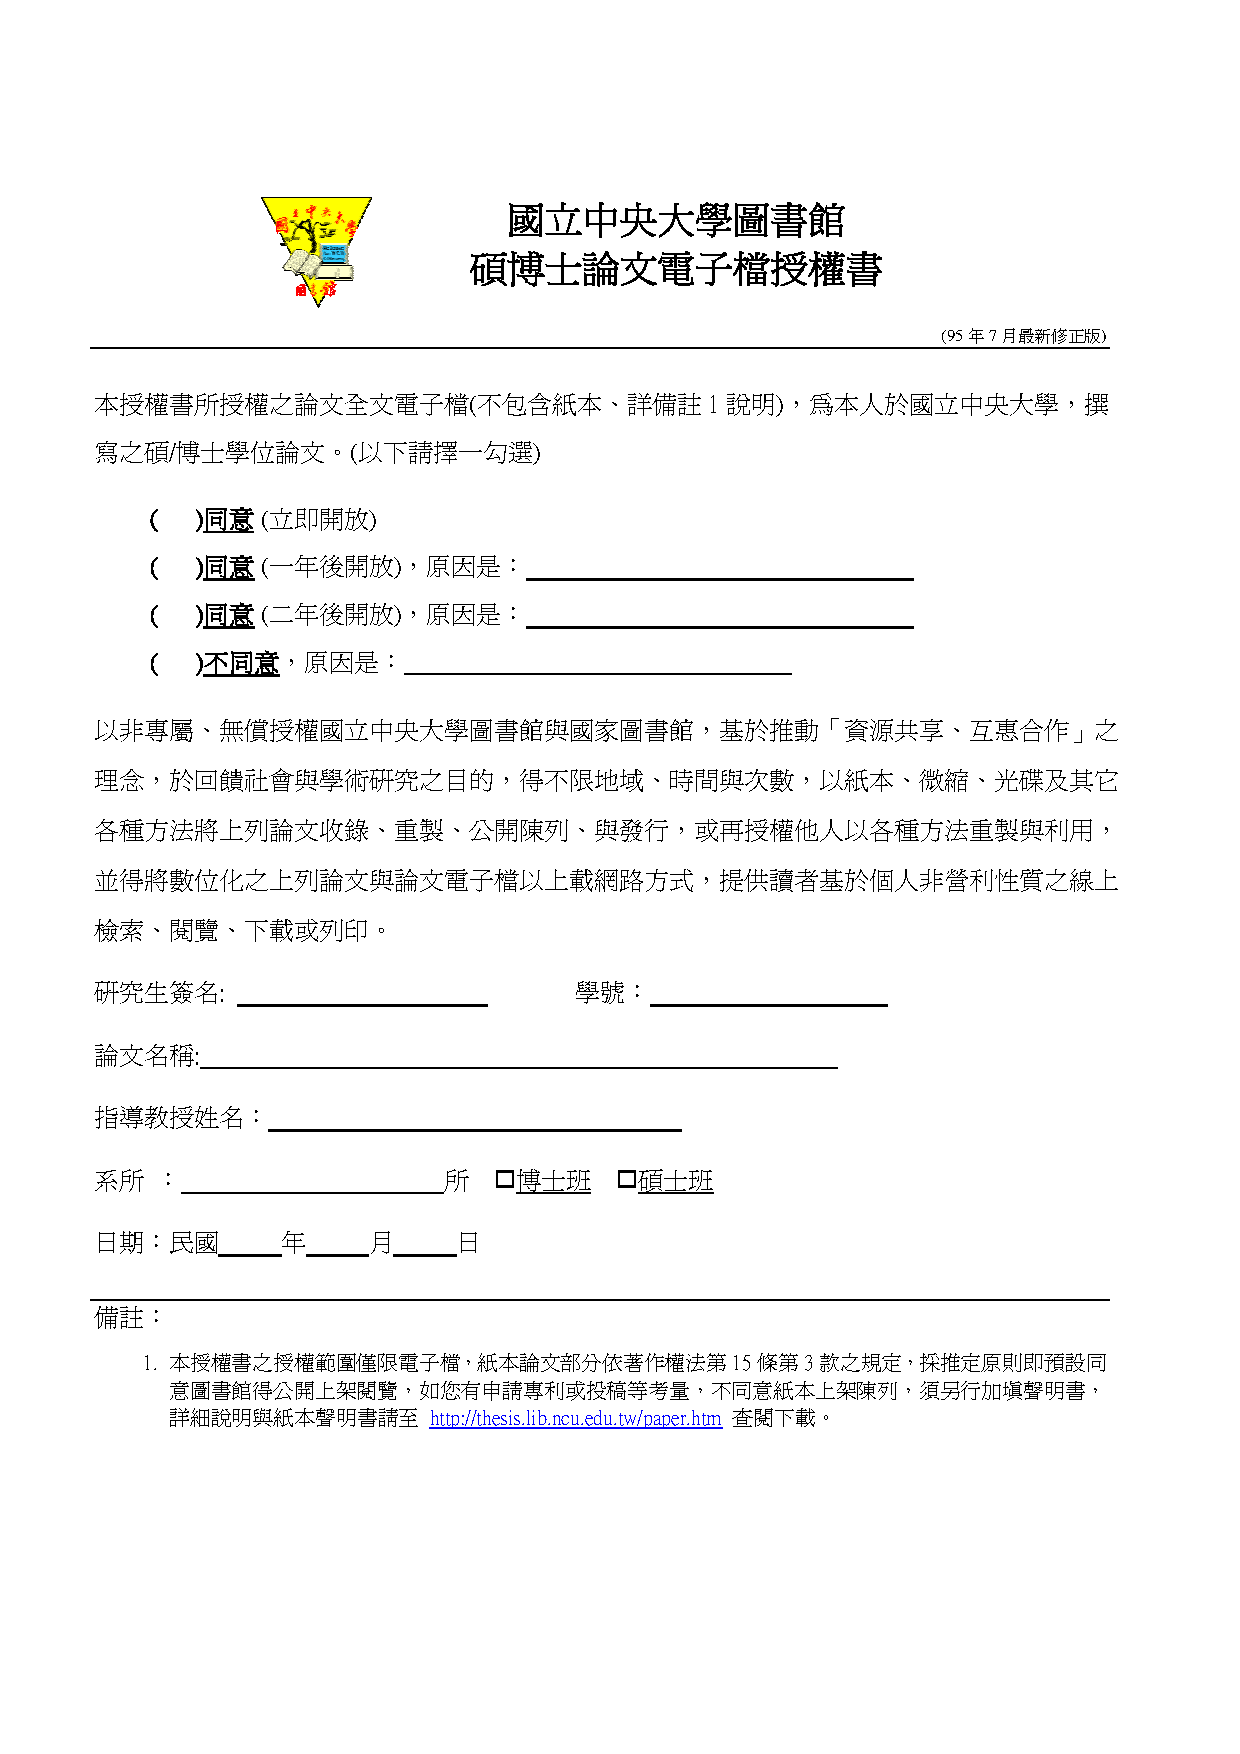
\includepdf[pages=-,scale=0.9]{myfile.pdf} % 插入其他表格
\cleardoublepage                 % \frontmatter
\pagenumbering{roman}            % 羅馬數字編頁
\begin{abstractcn}
\index{ncuthesis 環境!abstractcn}


關鍵字: 碩博士論文,體裁檔,\LaTeX
\vspace{2em}

此論文範例得以完成是由於體裁檔({\tt ncuthesis.cls})的完成。期間多方閱讀、吸收、漸有所獲,直至發掘兩篇網路文章,深入了解後再加入中文化及適當增修而成。本體裁檔可再增修,複製,直接採用做個人用途,或供單位使用,唯不可做商業用途。

此套件係自助編寫屬非賣品,可自由使用,但不做任何保證。期望提供學生便利性,做出符合國立中央大學所規範的研究所論文格式,但不隱含任何商業價值。\href{./form03-02-02.doc}{Open NCU Thesis Requirements}
\begin{center}
功能
\end{center}
\begin{itemize}
\item 論文格式滿足本校要求。
\item {\tt Uncode/UTF8} 中文化。
\item 可選擇編譯方式(pdf\LaTeX,Xe\LaTeX)。
\item 可選單面印刷或雙面印刷。
\item 快速編譯及越界偵錯。
\item 可列印紙張結構及參數。
\item 顯示智財權及製作日期。
\item 如何使用體裁檔請看第一章說明。
\item 如何使用\LaTeX\ 請看第二章說明。
\item 如何製作參考文獻請看第三章說明。
\item 具索引(index)功能。
\end{itemize}
\end{abstractcn}              % 中文摘要abstractcn環境
\begin{abstracten}
\index{ncuthesis 環境!abstracten}

{\bf \sf Keywords:} Master/Doctorial thesis, Class file, \LaTeX, \XeLaTeX

\vspace{2em}

The files included in the directiory are free to use, copy, or modify for personal use or within an organization. Primarily, the files are for graduates who want to write their theses in \LaTeX/\XeLaTeX{} and meet the requirements stipulated by the National Central University.

This document is distributed in the hope that it will be useful to graduates, but without any warranty; without even the implied warranty of merchantability.
\begin{center}
Source\\
\url{https://code.google.com/p/ncu-thesis-latex-template/}\\
Features
\begin{itemize}
\item Master/Doctorial thesis stipulated by National Central University. 
\item Unicode/UTF8 supports.
\item Compilable by pdf\LaTeX{ } or \XeLaTeX. 
\item Oneside or twoside printing.
\item Fast compilation and overfull detection. 
\item Page layout and parameters.
\item Copyright and time stamp.
\item Index, watermark capabilities.
\item Other thesis variants and todonote reminder.
\item How to use this package $--$ Chapter 1.
\item How to use \LaTeX\ (very brief) $--$ Chapter 2.
\item How to generate references $--$ Chapter 3.
\end{itemize}
\end{center}
\end{abstracten} 

             % 英文摘要    abstracten
\begin{acknowledgements} \index{謝誌}
\index{ncuthesis 環境!acknowledgements}

體裁檔受啟發於兩位英美教授於網路上的文章,並經吾人中文化及適當增修而成。本體裁檔可再增修,複製,直接採用做個人用途,或單位使用,唯不可做商業用途。請尊重上述兩位教授的無私奉獻。

\begin{itemize}
\item 感謝\TeX/\LaTeX{}網路社群內,龐大的\TeX/\LaTeX 社群及其網頁提供無價資訊。
\item 欣逢中央大學教務處註冊組組長,蕭嘉璋老師,見微知著,並予協助,僅此誌謝。
\item 承蒙太空及遙測研究中心蔡富安老師協助在{\tt Ubuntu 12.04上TeXLive-2009}測試成功,僅此誌謝。
\item \texttt{2013/06/13}碩士班 葉信麟同學發現目錄頁碼不正確。
\end{itemize}
\end{acknowledgements}             % 謝誌        acknowledge
\phantomsection\addcontentsline{toc}{chapter}{目錄}
\tableofcontents                 % toc
\phantomsection\addcontentsline{toc}{chapter}{圖目錄}
\renewcommand{\numberline}[1]{圖~#1\hspace*{1em}}%圖目錄
\listoffigures                   % lof
\renewcommand{\numberline}[1]{表~#1\hspace*{1em}}%表目錄
\phantomsection\addcontentsline{toc}{chapter}{表目錄}
\listoftables                    % lot                  % 目錄  toc, lof, and lot
\begin{symbols}
\index{ncuthesis 環境!symbols}
\begin{tabular}{l@{ : }l}
\textbackslash dept & {研究所}           \\[1ex]                         
\textbackslash degree & {碩/博士 or 專題研究 or 論文計畫書}     \\[1ex]                                      
\textbackslash title & {論文中文題目}  \\[1ex]
\textbackslash subtitle & {論文英文題目}  \\[1ex] 
\textbackslash logo & 封面校徽(預設中央校徽)\\[1ex]
\textbackslash author& 作者             \\[1ex]                                   
\textbackslash mprof&  指導教授          \\[1ex]                  
\textbackslash sprofi, \textbackslash sprofii& 兩位共同指導 \\[1ex]
\textbackslash degreedate& 中~華~民~國~XXX~年~X~月 \\[1ex]
\textbackslash copyyear& 著作完成年  \\[1ex]
\textbackslash includepdf & 插頁指令,需pdfpages巨集 \\[1ex]
\textbackslash fontsize\ldots\textbackslash selectfont & 設定字大小行距\\[1ex]
\textbackslash bookbone & 書脊短時用\\[1ex]
abstractcn & 中文摘要環境名,檔案則為abstractcn.tex\\[1ex]
abstracten &  中文摘要環境名,檔案則為abstracten.tex\\[1ex]
acknowledge{\color{red}ments} &  謝誌環境名,檔案則為acknowledge.tex\\[1ex]
append{\color {red}A} &  附錄一環境名,檔案則為appendix.tex\\[1ex]
append{\color {red}B} &  附錄二環境名,檔案則為appendix.tex\\[1ex]
symbol{\color {red}s} &  符號說明環境名,檔案則為symbol.tex\\[1ex]
\end{tabular}
\label{symb}
\end{symbols}                 % 符號說明   symbols 環境
\cleardoublepage
\index{\LaTeX!\textbackslash include}
\pagenumbering{arabic}           % 阿拉伯數字編頁
                                 % \mainmatter
\chapter{使用說明}

多年來研究室碩士班學生雖以\LaTeX 撰寫論文,文章結構多引用前屆學長論文結構,然共同的體裁檔一直欠缺,今從網路學習各校之體裁檔,加以正值著作期間,不斷瀏覽,收尋相關網頁,獲致許多相關知識,故解決多年困擾有望。此論文範本將{\tt ncuthesis}的使用說明以五章來陳述並做成中央大學標準論文格式,原始碼與PDF輸出皆放在''{\tt NCU}論文"的檔案夾內。請看{\tt README}說明於第三章內,其實只有三章重點,基於彰顯論文結構而將較不重要的小節亦以章的結構出現。
\begin{itemize}
\item {\color{red}紅色} ---  非常重要,因人而需修改。
\item {\color{blue}藍色} --- 必備知識,因需要而採用。
\end{itemize}
\index{ncuthesis 體裁!ncuthesisXe}\index{ncuthesis 體裁!ncuthesisCJK}
\section{文獻回顧}
此碩博士論文之體裁檔受啟發於兩位英美教授於網路上的公開文章與檔案
\begin{enumerate}
\item Class file: ociamthesis v2.2 (22/11/2010) \\
    By Keith A. Gillow $<$gillow@maths.ox.ac.uk$>$. \\
    Version 1.0 released 26/11/1997\\
	\url{http://www.maths.ox.ac.uk/help/faqs/latex/thesisclass}
\item "Minutes in less than Hours: Using \LaTeX\ Resources" \\
    by Jim Hefferon, $<$ftpmaint@tug.ctan.org$>$\\
	\url{http://tug.org/pracjourn/2005-4/hefferon/}
\end{enumerate}

\section{研究動機}
前述兩位教授的無私奉獻,進而激發自行學習撰寫體裁檔的願望。逢此畢業時節,最需要的體裁檔就屬符合中央大學碩博士論文的\LaTeX{}/\XeLaTeX{}體裁檔;在歐美國家,很多公、私立大學,都有屬於各校的檔案在網路上提供學生另一種選擇,讓研究生在低阻力,高效率下,輕鬆地做出字型美,排版佳,品質高,檔案小且全校統一的論文。然經網路搜尋後,中央大學無此資源與學生共享。心想,若撰寫成功則學生受惠,個人則增長知識且實驗室將有一致且符合校方要求的論文格式。

\section{研究目標}
撰寫體裁檔的目標是學生不需擔心論文設定問題。一切都由體裁檔負責。故其設計內容含 \par
\begin{table}[!hbt]
\centering             \index{\LaTeX!\textbackslash centering}
\caption{研究目標}
\begin{tabular}{cccccc}\\
論文封面 & 設定長寬 & 章節目錄 & 書脊文字 & 超連結 & 插頁技巧\\ 
編製頁碼 & 摘要附錄 & 字體行距 & 中文書籤 & 中文化 & 浮水印記\\
兩種編譯 & 多功選項 & 多種文書 & 程式撰寫 & 投影片\\
\end{tabular}
\end{table}

	準此,以上設定都以中央大學論文要求為準,至於其它大專院校論文格式\footnote{上網收尋並予此手冊比較。}應可自行修改,本手冊有提供修改方式及例題\footnote{其實97\%相同,不同在封面結構,摘要,與有無浮水印。},學生不須操心,認真閱讀、了解後自然會修改。
\section{中文化}
首先需中文化,此體裁檔採用國際上常用的兩種(亞洲字型,電腦內含字型)中文化結構:
\begin{itemize}
\item {\tt CJK (Chinese Janpanese Korean)}中文化: 使用pdf\LaTeX編譯。 
\begin{enumerate}
\item 使用{\tt titlesec, titletoc}處理章次及目錄。
\item 中文化相關巨集
{\tt CJKutf8,CJKvert,CJKnumb, fancyvrb},
{\tt verbatim, pdflscape, titlesec, titletoc} 已自動載入。不須再另行載入。
{\tt mypreamble.tex} 則提供其他讀者自訂巨集例如 
{\tt amssymb},{\tt amsmath,background,circuitikz}等,端視讀者需求。

\index{Packages!background}\index{Packages!tikzpicture}
\index{中文化!CJKutf8}\index{中文化!CJKvert}
\index{中文化!titletoc}\index{中文化!titlesec}
\index{中文化!CJKnumb}

\item 用 {\tt pdfLaTeX+MakeIndex+BibTeX}編譯。
\item 主檔案為{\tt masterthesis{\color{red}CJK.tex}及ncuthesis{\color{red}CJK}.cls}。
\end{enumerate}

\item {\tt xeCJK} 中文化: 使用\XeLaTeX編譯。\index{中文化!xeCJK}
\begin{enumerate}

\item 修改{\tt report class 內\textbackslash\char64chapter, \textbackslash\char64makechapterhead}處理章次及目錄。

\item 中文化相關巨集 
{\tt xltxtra,xunicode,CJKnumb,fancyvrb},
{\tt verbatim} 已自動載入。不須再另行載入。{\tt mypreamble.tex} 則提供其他讀者自訂巨集例如
{\tt amssymb,amsmath},{\tt background},
{\tt circuitikz}等,端視讀者需求。

\index{中文化!xltxtra}\index{中文化!xunicode}
\item 用{\tt XeLaTeX+MakeIndex+BibTeX}編譯。
\item 主檔案為{\tt masterthesis{\color{red}Xe.tex}及ncuthesis{\color{red}Xe}.cls}。
\end{enumerate}
兩種主檔案兩者不同之處其實只有10行左右。但為方便不同的研究生使用,故刻意做出兩份。雖然台灣有其他 $\chi$\TeX({\tt aka. chi\TeX}),cw\TeX,PU\TeX的相同軟體,但編譯時可能有兩種中文相衝的可能性,未深入研究。
\end{itemize}

\section{論文結構}
稍微了解\TeX{}/\LaTeX\ 的學生讀者應可了解下列結構,因為是沿用\LaTeX\ {\tt report}結構。只是體裁檔{\tt (class file)}需寫入{\tt ncuthesisCJK}\hfil\break或{\tt ncuthesisXe}以便做出符合中央大學範例的格式。%
\index{\LaTeX!classes!report}\index{\LaTeX!classes!article}
\index{\LaTeX!\textbackslash chapter}\index{\LaTeX!\textbackslash section}\index{\LaTeX!\textbackslash subsection}\index{\LaTeX!\textbackslash subsubsection}\index{\LaTeX!\textbackslash author}\index{\LaTeX環境!table} \index{論文結構}
\label{bookstruc} \index{\LaTeX!\textbackslash label}
\begin{table}[hbt!]
\caption{論文結構}
\end{table}
\fvset{frame=topline,numbers=left,numbersep=3pt,
firstline=1,lastline=1}
\VerbatimInput{masterthesisXe.tex}
宣告區\quad {\tt Preamble}
\fvset{frame=topline,numbers=left,numbersep=3pt,
firstline=22,lastline=22}
\VerbatimInput{masterthesisXe.tex}
本文區\quad {\tt Text body}
\fvset{frame=bottomline,numbers=left,numbersep=3pt,
firstline=52,lastline=52}
\VerbatimInput{masterthesisXe.tex}

\index{\LaTeX!\textbackslash VerbatimInput}
此資料夾提供兩種中文化方法,使用時先選擇主檔(建議\XeLaTeX\ 編譯方式),然後將{\tt masterthesisCJK.tex} 或 {\tt masterthesisXe.tex} 另存新檔,給一個自己喜歡的檔名譬如{\tt foo.tex}。新檔內容幾乎一模一樣不需改變甚麼(所以簡單吧)。但是至少系所、學生、教授、論文題目不同,須修正,現將分別陳述於後: \index{\LaTeX!\textbackslash input}
\index{Packages!verbatim}\index{foo}

\subsection{宣告區}

\fvset{frame=single,numbers=left,numbersep=3pt,
firstline=2,lastline=5}
\VerbatimInput{masterthesisXe.tex} 
\index{\LaTeX!\textbackslash VerbatimInput}
宣告區內2-3行是本檔使用的外來巨集(必要具集則在{\tt*.cls}內)。
\fvset{frame=single,framerule=1mm,numbers=left,numbersep=3pt,
rulecolor=\color{red},firstline=6,lastline=16}
\VerbatimInput{masterthesisXe.tex} 
6-16行是系所、學位、論文題目\footnote{亦可填入非學位性的研究計畫,讀書計畫等。}、研究生、指導教授可照論文範例填入相關資訊。共同指導教授(預設是無)亦可填二位。\index{宣告區}
\index{ncuthesis 指令!\textbackslash mprof} \index{ncuthesis 指令!\textbackslash sprof} \index{ncuthesis 指令!\textbackslash sprofa}
\index{ncuthesis 指令!\textbackslash title} \index{ncuthesis 指令!\textbackslash subtitle}\index{ncuthesis 指令!\textbackslash degree} \index{ncuthesis 指令!\textbackslash degreedate}\index{ncuthesis 指令!\textbackslash author}
\index{ncuthesis 指令!\textbackslash copyyear}\index{ncuthesis 指令!\textbackslash dept}%
\fvset{frame=single,framerule=0.4pt,numbers=left,numbersep=3pt,
rulecolor=\color{black},firstline=17,lastline=21}
\VerbatimInput{masterthesisXe.tex} 
17行是自行定義的中文化定理、引理、例題等具重複性常用定義。
如果自訂巨集少則自行加入,若多則建議寫入{\tt mypreamble.tex},再以\textbackslash {\tt input}引入。如範例所示。 第21行則是要求索引製作。
\index{ncuthesis 檔案!mypreamble}\index{ncuthesis 檔案!ncuthesisCJK}\index{ncuthesis 檔案!ncuthesisXe}\index{ncuthesis 檔案!abstractcn}\index{ncuthesis 檔案!abstracten}
\index{ncuthesis 檔案!chapter1}\index{ncuthesis 檔案!chapter2}\index{ncuthesis 檔案!appendA}\index{ncuthesis 檔案!appendB}\index{ncuthesis 檔案!bibli}\index{ncuthesis 檔案!symbol}\index{ncuthesis 檔案!acknowledge}
\index{Packages!calculator}\index{Packages!showframe}
\index{Packages!hyperref}\index{Packages!fancyvrb}

\subsection{本文區}
\fvset{frame=single,numbers=left,numbersep=3pt,firstline=23,lastline=32}
\VerbatimInput{masterthesisXe.tex}
這些行是製作封面,書名頁,非\LaTeX{}格式但已成為PDF格式紙張插頁,例如各校口試委員簽名頁等畢業有關之頁。

\fvset{frame=single,framerule=1mm,numbers=left,numbersep=3pt,
rulecolor=\color{blue},firstline=33,lastline=39}
\VerbatimInput{masterthesisXe.tex}
35-39行依序為中英文摘要、謝誌、目錄、圖目、表目、符號說明等。 因論文需要而設計的特定環境(不需要則不必寫,用\%使其\textbackslash include指令無效)。\index{\LaTeX環境!tabbing}

\index{ncuthesis 環境!abstractcn} \index{ncuthesis 環境!abstracten}\index{ncuthesis 環境!acknowledgements} 
\index{ncuthesis 環境!symbols}\index{ncuthesis 環境!appendA}\index{ncuthesis 環境!appendB}

\fvset{frame=single, framerule=1mm,numbers=left,numbersep=3pt,
rulecolor=\color{blue},firstline=40,lastline=48}

\VerbatimInput{masterthesisXe.tex}
第43-48行用\verb|\include|加入其他各章節,是屬\LaTeX的用法,如同打字一般,將文字內容打入各檔案。第二章有簡要說明\LaTeX用法。
48行是參考文獻設定。本書用簡單的方式,另有檔案方式({\tt.bib}),請看第二章。

\fvset{frame=single,framerule=0.4pt,numbers=left,numbersep=3pt,
rulecolor=\color{black},firstline=49,lastline=51}
\VerbatimInput{masterthesisXe.tex}
49-51行是為了了解紙張設定,可除去(\%)不用。

\subsection{插頁}
本論文封面已設計成中大碩博士論文封面,然因中央大學有其它表格化的{\tt doc}檔,此手冊並未以\LaTeX設計其相關表格,以維持與其他學校論文架構最大的相容性,方便推廣至其他大專院校。然如何加入特定表格?建議用插頁方式如下。先完成{\tt DOC}相關表格\todo[inline]{此表格學生需自行確認是最新版},排好順序,再存成{\tt myfile.pdf}檔,其中每一頁之後皆要插入空白頁,才能保證出現在奇數頁。所以若有非\LaTeX的{\tt pdf}檔皆可以類推,加入論文內。
\index{ncuthesis 檔案!committee}
\begin{verbatim}
1. \usepackage{pdfpages}    % 於宣告區
2. 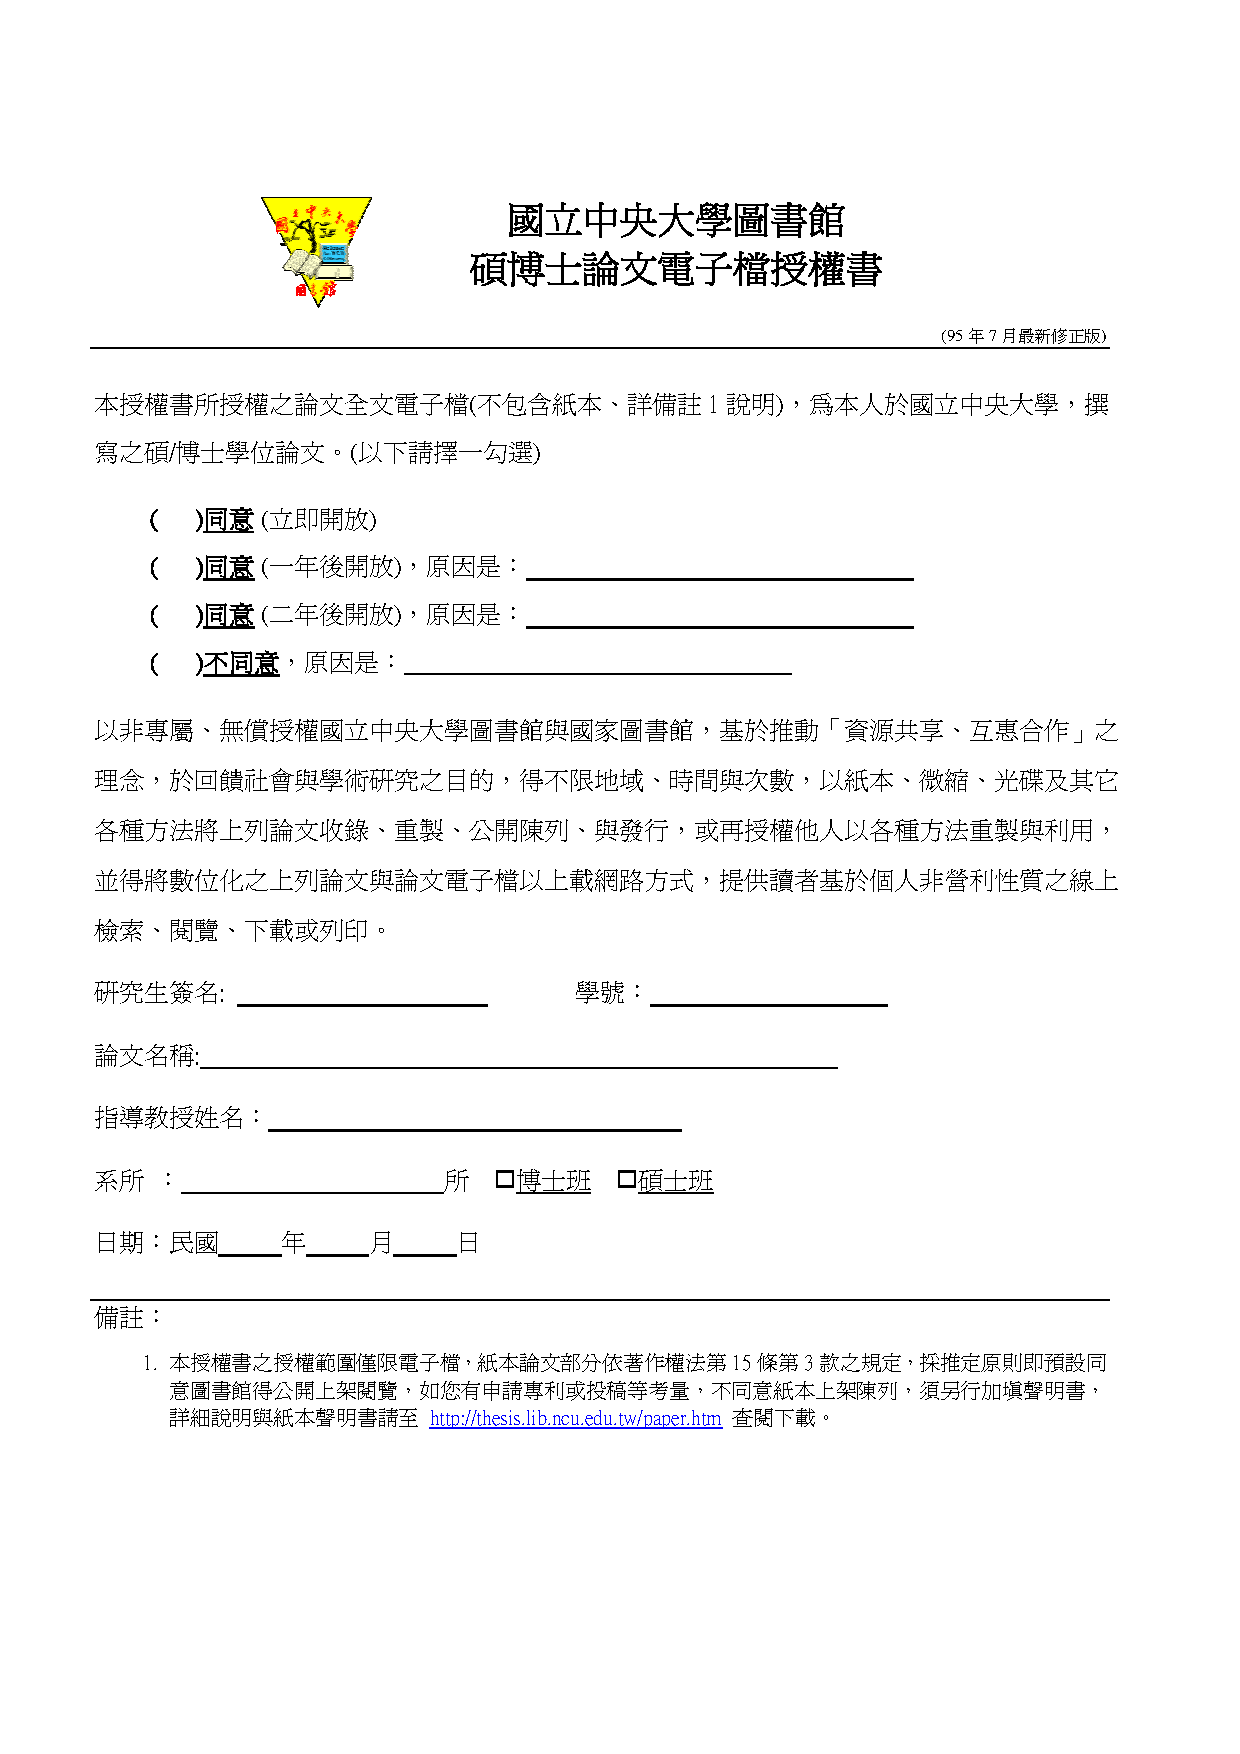
\includepdf[pages=-,     % - =所有頁面 或用 1,2 表示
      addtotoc={1,subsection,2,{書簽名},標名}]{myfile.pdf}
註解:addtotoc={page number,section,level,heading,label}
\end{verbatim}

第1行寫於宣告區。插頁若需出現在目錄則加{\tt addtotoc}指令。上述之第2行於插頁需要之處寫入。如本例第32行所示,再次顯示於下:
\fvset{frame=single,framerule=1mm,numbers=left,numbersep=3pt,
rulecolor=\color{blue},firstline=32,lastline=32}
\VerbatimInput{masterthesisXe.tex}

另外有些博士生將履歷 ({\tt via package moderncv}) 加入論文最後幾頁,亦可用此技巧達成。所以只要是非以\LaTeX產生的圖表轉成{\tt png,jpg,jpeg,pdf}檔後,皆可依此方式加入論文並與論文成為一體自動連號。

\section{結語}
簡而言之,此論文的主檔案有兩類
\begin{itemize}
\item {\tt masterthesisCJK.tex} 及必需之體裁檔 {\tt ncuthesisCJK.cls}
\item {\tt masterthesisXe.tex } 及必需之體裁檔 {\tt ncuthesisXe.cls}
\end{itemize}
提供論文編寫方式,其輸出即是標準格式。快速、方便、及時。
\index{\LaTeX環境!itemize}
\begin{itemize} \index{\TeX!\LaTeX}
\item 本論文假設學生有 \TeX/\LaTeX 基礎知識,若需加強相關知識,網路上有免費資訊可供學習。第二章亦提供一些入門知識及參考網址。 \index{使用手冊}

\item 第20行:可只編譯某些檔(以逗點分開),除錯時好用,可降低編譯時間。
\fvset{frame=single,numbers=left,numbersep=3pt,
rulecolor=\color{blue},firstline=20,lastline=20}
\VerbatimInput{masterthesisXe.tex}

\item 第25行:中文字大小及行距是由這行設定
\fvset{frame=single,numbers=left,numbersep=3pt,
rulecolor=\color{blue},firstline=25,lastline=25}

\VerbatimInput{masterthesisXe.tex}

\item 使用亞洲字型{\tt CJK,xeCJK}中文化且設定為楷書({\tt bkai}),不是 cw\TeX 或 PU\TeX 或 $\chi$\TeX。 \index{\TeX!cw\TeX}\index{\TeX!PU\TeX}

\item 使用時需有{\tt unicode/utf8}編輯器如{\tt MiKTeX的TeXworks}\footnote{LyX愛好者可先將檔案({\tt chapter1,2,3...})做好再存成{\tt .tex}檔然後用{\tt masterthesis.tex}編譯}。 \index{MiKTeX}\index{TeXworks} \index{\TeX!LyX}\index{\TeX!\XeLaTeX}

\item {\color{red}行動安裝}在第二章說明,{\tt Window/Android}版免費排版系統\linebreak \TeX{}/\LaTeX{}/\XeLaTeX{}垂手可得,亦建議採用。 

\item 使用pdf\LaTeX或 \XeLaTeX連續編譯兩次({\tt TeXworks} 會自動執行兩次)。故若有圖檔請都存成{\tt png, jpg, jpeg, pdf}。

\item 撰寫方式如\TeX/\LaTeX{}一般寫作技巧。此範例主要是用環境\linebreak({\tt environment}) 技巧。除"\,附錄"環境外,所有其他環境皆會自動帶入論文題目。\label{indpage}

\item {\color{red}論文很少用索引,故{\tt makeidx,\textbackslash makeindex,\textbackslash printindex}三指令(第2、34行,最後一行在{\tt bibli}內) 可省略,但此論文範本保留,以便保有科技書籍的格式,請看第\framebox{\pageref{others}}頁。}

\item {\tt bookbone.tex}提供製作論文書脊,現印於右側以便觀察 (\XeLaTeX{}則無法呈現!?) 
長書脊時請仿照校名({\tt tabular}技巧)製作兩欄式,只要單獨編譯{\tt bookbone.tex} 即可得。 \index{ncuthesis 指令!\textbackslash backbone}
%\marginpar[\includegraphics{bookbone.pdf]{}

\item 本論文用到的輸入參數整理在符號說明頁。了解後就可開始用此套件了。\label{conclude}

\item 編譯時,可選單面印刷(預設值)或雙面印刷: \index{\LaTeX!\textbackslash noframe}%
單面印刷({\tt oneside}) -- 適合一般計畫({\tt project})或報告({\tt report})。\\
雙面印刷({\tt twoside}) -- 適合正式文件({\tt thesis}),有封面,謝誌等。
\item 另外有四種工作模式可選擇:\\ \index{\LaTeX!\textbackslash draft}
\index{\LaTeX!\textbackslash marginnote} \index{\LaTeX!\textbackslash raggedright} 
\index{\LaTeX!\textbackslash raggedleft}
{\color{blue}
\begin{center}
\begin{tabular}{|c|c|c|} \hline 
 選項          &  空白    &  {\tt  draft}      \\ \hline 
 空白          &    框    &    框 +頁眉      \\ \hline
{\tt noframe}  &    無框  &    無框+頁眉   \\ \hline
\end{tabular}
\end{center}
}
空白是單頁印刷({\tt oneside}),因為是預設值。若改為{\tt twoside}則為雙頁印刷,故單面印刷有四種,雙面印刷又重複四種。

\begin{enumerate}
\item $<$空白,空白$>$此預設值會產生文字外框,偵測是否越界。
\item $<${\tt draft},空白$>$選項,編譯較快,圖形或插頁皆以方格表示並不載入,且右邊會出現黑體垂線表示超出頁面範圍,方便修改除錯。且頁眉右側會出現智財權屬於作者,以防止文件不慎遺出。
\item$<$空白,{\tt noframe}$>$除去外框之{\color{red}單頁印刷完稿},要雙頁印刷之完稿,別忘了要用{\tt twoside}{\color{red}。的確,$<${\tt twoside,noframe}$>$才是最後完稿。}\todo[inline]{切記!切記! [disable] for removing todos, [twosides, noframe] for final version。}但有些學校論文少於100頁可採單頁印刷。


\item$<${\tt draft,noframe}$>$無外框但有頁眉。
\end{enumerate}
\item \textbackslash printpapersize 會印出目前頁面參數。
{\tt ncuthesisXe.cls}檔案內第51-57行(請參看附錄一),可改變紙張大小。\\
\framebox{
\printpagesize 
}\\               % to print page size
上示參數為相對於紙張左上角(視為原點),向右向下(1in,-1in)處之參考點。\index{ncuthesis 指令!\textbackslash printpapersize}
\item \LaTeX有五種體裁檔{\tt article, book, report, letter, slides}\hfil\break{\tt ncuthesisXe(CJK)}則是結合{\tt report}再定義新環境而成。故要產生本校的固定格式必需用{\tt ncuthesisXe(CJK)}。\index{\LaTeX!\textbackslash hfil}
\index{\LaTeX!classes!article}\index{\LaTeX!classes!book}\index{\LaTeX!classes!report}
\index{\LaTeX!classes!letter}\index{\LaTeX!classes!slides}
\item 浮水印的程式碼在{\tt mypreamble.tex}內,需{\tt background}套件(手冊);不需要者可用(\%)除去。中央大學不需浮水印,但設計它的原因是(1)可放大改成時間或加入防拷貝字語,(2)可置於頁面任何位置(包含斜放),(3)其他學校(清大,台科大,北科大)有浮水印需求。\index{watermark}\index{浮水印}
\item 論文寫作的過程中,常常需要自我提醒,要修改這,修改那,要加入圖表等代辦事項。這時我們可用\verb|\todo[inline]{提醒內容}|\todo[inline]{提醒內容}立即於寫作的同時加入,它會以橘色顯示在論文中以免忘記。這些提醒事項都會收錄在單頁{\tt List of todos}中,一目了然,非常好用。當然完稿時,切記要以{\tt \textbackslash usepackage[disable]\{todonotes\}}除去所有提醒、代辦事項;不然你的論文有很多代辦事項卻是正式文件。
\end{itemize}

\section{其他文書\label{others}}\index{其它文書}

此一節是為了想了解如何修改程式碼的讀者而寫的,尤其是非中央大學的研究生。例如 (1)某大學的研究生也想使用此套件來寫論文,但中央格式與該校不同;(2) 某研究生想為該校寫出適合該校的\LaTeX碩博士論文套件,並發表於網路上且會維護它; (3) 想進一步學習\LaTeX基礎者,則須研究本節。所以不是這目的的讀者可跳過這一節。

此檔案夾可製作的文書不止論文而已,其實只要稍微增修就可產生很多其他文書結構。各行各業中常見的文書有

\begin{itemize}
\item 書 --- 封面、摘要、章節、附錄、索引、文獻。

以論文首頁做為書的封面較罕見,大部分需牽涉封面設計,故此頁需請專人設計。其實\LaTeX的封面設計({\tt book design})可自己設計,需上網學。

\item 論文 --- 首頁、摘要、章節、附錄、文獻。

這是此手冊的主要目標。其它大專院校論文格式需自行更改,其實論文主體(目錄、章節、附錄、索引、文獻) 因教育部法規已定,各校一致性頗高,剩下的約十頁左右,有明顯差異(例如中英文摘要多了姓名及系所)。故根據下列方向修改,各校論文99\%的吻合度是可達成的。
\begin{itemize}
\item 封面格式:{\tt ncuthesis.cls}檔,約在{\tt 167-202}行。
\begin{itemize}
\item [1] 熟悉\LaTeX者可直接修改。\index{\LaTeX!\textbackslash titlepage}
\item [2]  自動化  以{\tt \textbackslash (re)newcommand}定義指令{\tt \textbackslash commands},請參考附錄二。

\item [3] 手動化 用{\tt titlepage}環境撰寫,請參考附錄二。

\item [4] 以{\tt doc}製作封面後轉成{\tt pdf}以取代中央封面,此法最快,但\LaTeX均質性較差。其實{\tt myfile.pdf}的目的即是為此而設計。
\end{itemize}
\item 中英文摘要:亦可類推。這部分是各校差異所在。附錄二亦有用\verb|\renewenvironment{onecol}|修改,可參考附錄二。

\item 紙張大小:都是{\tt A4}紙張,但內文四周留白寬度可能稍微不同,這可由{\tt ncuthesis.cls}檔內修改,約在{\tt 51-57}行。
\item 字體索引:詳見第\fbox{\pageref{indpage}}頁。
\item 去浮水印:{\tt mypreamble.tex}內,刪除相關指令。
\item 章節標題:本校用中文數字一、二、三為章次編號,有些學校則用第一章,第一節來編號,欲改為後者可將{\tt ncuthesis.cls}內第{\tt 85}行加入兩中文字,改\verb|\CJKnumber{\arabic{chapter}}、|改為
{\color{red}第}\verb|\CJKnumber{\arabic{chapter}}|{\color{red}章},餘類推。
\item 增加目錄:若要將"\,論文審定書"加入目錄,則加入下列兩行於審定書之前即可,餘類推。
\begin{verbatim}
\cleardoublepage\phantomsection     % 強制奇數頁開始
\addcontentsline{toc}{chapter}{論文審定書}% 加入目錄
其中 chapter 亦可改為 (sub/sub)section.
\end{verbatim}
\end{itemize}

\item 報告(論文計劃書) --- 首頁、摘要、章節、附錄、文獻。

報告稍微正式,故封面可沿用論文封面。

\item 作業 --- 首頁、章節。\index{其它文書!作業}

首頁 改寫 姓名、學號、班級、科目,如果希望不要單獨一張封面(因較非正式或浪費),請參考附錄二。


\item 會議記錄

如作業範例所示,稍微修改上半部的內容及將"\,作業環境"改為"\,議題環境"即可。要更正式一點,請看文獻回顧第二篇
。\framebox{Back\pageref{conclude}}
\end{itemize}

\section{編譯失敗}
目前,此體裁檔在六台不同的電腦(皆{\tt Windows})及一台{\tt Ubuntu上安裝LyX2.0.2/TeXLive2009},測試成功,都是安裝英文\LaTeX{},沒有中文化的cw\TeX,PU\TeX,$\chi$\TeX。一般來說,不會有問題。但若編譯失敗,請試試看下列建議。
\begin{enumerate}
\item 編譯時若錯誤訊息顯示和{\tt .aux} 有關,請清除所有{\tt *.aux}檔案。因為兩種編譯方法使用同一檔案夾,有可能相衝。 
\item 第一步測試結果問題仍然在,可能是中文相衝。測試的電腦其\LaTeX{ }系統是否有安裝 $\chi$\TeX,cw\TeX或PU\TeX嗎?本論文製作時是在英文\LaTeX{}下加 {\tt CJK/xeCJK}環境。建議試試看前述之{\tt USB}行動安裝,再執行編譯應可解決(換言之,單獨一個\LaTeX系統)。
\item {\color{red} 在{\tt USB}執行時,若找不到\LaTeX,請確認{\tt TeXworks}內指向正確 --- 
請檢查{\tt edit/preferences/typsetting/}+(新增)/{\tt USB}所在槽: \hfil\break
{\tt MiKTeX/miktex/bin}}。
\item {\color{red}編譯時 {\tt Acrobat reader} 請關掉,因{\tt TeXworks}有自己的閱讀器。}
\item 指令是否拼錯?錯一個字母都會產生除錯難度。
\item 編譯時,直接按{\tt enter}鍵,先忽略錯誤訊息,亦有助除錯。
\item 是否特定巨集({\tt macro})未放進來?\textbackslash usepackage\{\ldots\}未正確。
\item 將編譯的範圍縮小,試圖找出第一次就卡住的那段問題在何處?是否與數學符號有關,是否與表格或插圖有關?
\item 是否定義定理(\textbackslash newenvironment)或變數名{\verb|\def|}與{\tt ncuthesis}相同?
\item 任何問題,都可上網查詢。以{\tt Google}收尋"\,關鍵字"再加{\tt LaTeX}即可有很多知識等你學。這是\LaTeX迷人之處。
\end{enumerate}
               % 第一章    (自行寫入)
\chapter{\protect 語法入門}
首先,每章結構如下所示。

\begin{Verbatim}[frame=single,firstline=1,label=Every chapter]
\chapter{章名}           % 宣告某章開始
...
\section{節名一}         % 宣告某節開始
...
\section{節名二}
...
\subsection{小節名}       % 宣告小節開始
...
\subsubsection{小小節名}         % 宣告小小節開始
...
\end{Verbatim}
\index{Reserved words}
\begin{itemize}
\item 所有\LaTeX指令都由反斜線開頭,例如\textbackslash command (不可有{\tt arabic}數字)。
\item \LaTeX\ 保留字有十個: \textbackslash\  \$\ \{\ \}\ $\tilde{}$\ \#\ \%\ \&\ \textasciicircum\
 \_\ $>$, $<$ 不可單獨使用。  
\item \% 代表註解,其後任何字或空白皆忽略。
\item \LaTeX\ 一般檔案的副檔名為{\tt filename.tex},文獻檔則為\newline {\tt filename.bib}。其他都是編譯時產生輔助檔,可刪除。
\item 一個空白與連續數行的空白\LaTeX{}都是為一個空白,故主檔寫作時可適當留白,方便作者自行閱讀。
\item 環境名\textbackslash begin \ldots \textbackslash end,任何括號 $\{_1$ $[_2$ $(_{3}$ \ldots $)_3$ $]_2$ $\}_1$ 皆要對稱,不可錯置。
\end{itemize}
用{\textbackslash chapter\{章名\}}指令後,告訴\LaTeX{}以下文字要自成一章,就像打字一般,直接輸入中英文。
這樣就可以完成大部分的論文主體了。好用吧!!! 論文裡還有什麼
要寫?數學式啦!這是\LaTeX\ 的強項,我們稍後再說。先繼續介紹章節用法,這裡有假設、求解、驗證、數理基礎 四個小節({\tt section})。數理基礎又分次小節({\tt subsection})內含論文撰寫常用的技巧。

\section{假設}
若需要分章節則用{\textbackslash section\{節名\}},再繼續打字。
\section{求解}
同樣概念{\textbackslash section\{節名\}},繼續下去。若要換新的一章則開新檔{\tt chapter3.tex},內部第一行又如前所述

\section{驗證}
寫完後存檔。再以pdf\LaTeX\ 或 Xe\LaTeX\ 編譯。則可看到輸出。當然這一切都需在\TeX/\LaTeX環境之下。這方面知識網路很多。可自行上網學習。入門技巧約需1小時,主要是數學式寫法,現在我們將學一些初步技巧。
\section{數理基礎}
\index{\LaTeX!\textbackslash chapter}
\index{\LaTeX!\textbackslash section}
\index{\LaTeX!\textbackslash subsection} \index{\LaTeX\ 環境!Verbatim}%
數學式寫法很簡單,一行文字中含數學式是這樣寫\verb|$A^1_{234}$|,會產生文字中的數學式$A^1_{234}$,此例說明數學上下標的寫法,也說明有四個保留字不能亂用,因為保留給數學式\$\ 的上下標及群組概念了。數學式只能出現在文字內({\tt inline math mode})像這樣$1+\frac{1}{1+\frac{2}{1+\frac{3}{4}}}$,也不夠美觀。要單獨成一數學環境則用\\
\begin{Verbatim}[frame=single,firstline=1,label=Form 1 w/o number]
$$ 或 \[
1+\frac{1}{1+\frac{2}{1+\frac{3}{4}}}, \\
\frac{-b\pm\sqrt{b^2-4ac}}{2a}, \\
\quad \frac{a_1^{3x}+a_2^{-3x}}{a_1^x+a_2^{-x}}
$$ 或 \]
\end{Verbatim}
會單獨成一漂亮的數學式如下  \index{\LaTeX\ 環境!\textbackslash [}\index{\LaTeX\ 環境!\textbackslash ]}
$$ 
1+\frac{1}{1+\frac{2}{1+\frac{3}{4}}}, \\
\frac{-b\pm\sqrt{b^2-4ac}}{2a},\\
\quad \frac{a_1^{3x}+a_2^{-3x}}{a_1^x+a_2^{-x}}
$$
這樣就漂亮多了。注意在此數學環境強置換行(\textbackslash \textbackslash)無效,因結果是同一行印出,這一例題也說明
\begin{itemize}
\item 數學式有對齊的需要(聯立方程式)。
\item 適當留白亦有美觀效果,注意數學式間間距不同?如何達成\footnote{\textbackslash qquad,\textbackslash quad,\textbackslash ,\textbackslash,,\textbackslash;皆可,只是間距有別。}? 
\item 另外,但這樣寫是無編號的寫法,因為有時候我們需引用(\verb|\ref|)某方程式時則必須用編號的方式。
\end{itemize}
\index{\LaTeX\ 環境!\$\$}
\subsection{方程式}
最簡單的是用{\tt equation}環境,產生下列常微分方程式\\
\begin{Verbatim}[frame=single,firstline=1,label=Form 2 with number]  
\begin{equation}
\mbox{常微分方程式} \quad a \ddot y+ b\dot y +c=f
\label{eqn1}
\end{equation}
\end{Verbatim}
會產生 \index{\LaTeX\ 環境!minipage}
\begin{equation}
\mbox{常微分方程式} \quad a \ddot y+ b\dot y +c=f \index{\LaTeX!\textbackslash mbox}
\label{eqn1}
\end{equation}
文字環境有數學式用{\color{red}\$\mbox{math mode}\$}的方式表現。但數學環境中有文字時,用{\color{red}\verb+\mbox{text mode}+}表現。如上所示\footnote{其實\LaTeX\ 就是文字,數學,物件三大觀念,亦可混合一起使用。}。
而\verb|\label{eqn1}|是為了可稍後用{\verb|\ref{eqn1}|}參照。希望編號及間距的問題解決了,但希望對齊呢?要對齊則用{\tt eqnarray}環境及 \&\& (又一保留字)\\
\begin{Verbatim}[frame=single,firstline=1,label=Form 3 with alighment and number]
\begin{eqnarray}
f &=& a \ddot y+ b\dot y +c \nonumber \\
g &=& a\frac{\partial x}{\partial t_1}
+ b\frac{\partial x}{\partial t_2} +c
\end{eqnarray}
\end{Verbatim}
如上所示,其結果如下\footnote{強制換行在此環境有效。}。                \index{\LaTeX!\textbackslash ref}
\begin{eqnarray}
f&=& a \ddot y+ b\dot y +c \nonumber \\  \index{\LaTeX!\textbackslash nonumber}
g&=& a \frac{\partial x}{\partial t_1}
+ b \frac{\partial x}{\partial t_2}+c        % 最後一行不需 \\
\end{eqnarray}
結果是自動編號的對齊方式,有了數學式編號,但全篇都有用編號也不好,若不須編號則用\verb+\nonumber+加於該數式尾部\footnote{如果只要對齊,都不要編號則用\textbackslash begin\{eqnarray*\}/\textbackslash end\{eqnarray*\}。}
\index{\LaTeX\ 環境!eqnarray}

\subsection{矩陣}
矩陣則用{\tt equation}及{\tt array}環境,可印出如下所示。\index{\LaTeX\ 環境!equation}\\ 
\begin{Verbatim}[frame=single,firstline=1,label=Every matrix]
\begin{equation}
\left [              % 左 [
\begin{array}{ccc}   % c=置中,l=置左,r=置右。
a & b & 1\\
c & d & 2\\
4 & 5 & 6\
\end{array}
\right ]             % 右 ]
\label{mat1}
\end{equation}
\end{Verbatim}
會產生\footnote{不要編號的矩陣,怎麼寫? \qquad {\tt Ans:} \textbackslash [ \textbackslash ] or \$\$ \$\$。} \index{\LaTeX\ 環境!minipage}
\begin{equation}
\left [
\begin{array}{ccc}  \index{\LaTeX\ 環境!array}
a & b & 1\\
c & d & 2\\
4 & 5 & 6
\end{array}
\right ]
\label{mat1} \index{\LaTeX!\textbackslash label}\index{\LaTeX!\textbackslash ref}
\end{equation}
要引述前述之常微分方程式時則用 \verb|\ref{eqn1}|可把在前一頁的該方程式編號(\ref{eqn1})寫出,方便讀者理解所指方程式為何。同理,上一個矩陣亦可用\verb|\ref{mat1}|參照(\ref{mat1})。

下一個例題則是強調使用括號指令時需注意對稱的用法,\verb|\left \{|\footnote{注意:\{\}是保留字,要用它必須這樣用\textbackslash \{ \textbackslash \}} \ldots
\verb|\right .|。從結果可看出,用左大括號後並不需用右大括號,如何處理?如第8行所示。
\index{\LaTeX!\textbackslash footnote}

\begin{Verbatim}[frame=single,firstline=1,label=Pairs]
\begin{equation}
y=\frac{1}{x} \quad  
\left \{            % 左 {
\begin{array}{ll}   % c=置中,l=置左,r=置右
\frac{1}{x} & x \neq 0 \\  
\infty      & x = 0
\end{array}
\right .            % 右 } 不需要 則用此技巧
\end{equation}
\end{Verbatim}
\begin{equation}
y=\frac{1}{x} \quad  \index{\LaTeX!\textbackslash quad}
\left \{
\begin{array}{ll}   
\frac{1}{x} & x \neq 0 \\
\infty      & x = 0  \index{\LaTeX!\textbackslash neq}
\end{array}
\right .            
\end{equation}
\subsection{其他}
還有其他的數學式,例如\\
\begin{Verbatim}[frame=single,firstline=1,label=Various math forms]
\[
\sum_{i=1}^n A_i, \int_0^t f(\tau)\,d\tau, \sqrt{x}, \tan, 
\sin, \pi, \omega, f', \lim_{t\rightarrow \infty} f(t),
\forall x in \Re, \exists, \angle \theta, \bar A, \vec A
\]
\end{Verbatim}
可產生 \index{\LaTeX!\textbackslash sum} \index{\LaTeX!\textbackslash int} \index{\LaTeX!\textbackslash sqrt}
\[
\sum_{i=1}^n A_i,  \int_0^t f(\tau)\,d\tau, \sqrt{x}, \tan, \sin, \pi, \omega, f',
\lim_{t\rightarrow \infty} f(t),
\forall x \in \Re, \exists, \angle \theta, \bar A, \vec A
\]
以上是寫數學的技巧,因頁面限制無法全寫出來,為此,檔案夾內準備了一個網路上搜索來的檔案
\href{./Symbols.pdf}{ Symbols.pdf }內含所有數學式的寫法,方便各位寫數學式時參考。

\section{物件}
這裡是指數學定理,表格,小頁,列舉,插圖等獨立單元。
\index{\LaTeX!\textbackslash newtheorem}\index{\LaTeX!\textbackslash newcommand}

\subsection{定理}
主檔在宣告區有定義{\tt newtheorem}(用來定義使用者定理環境)中文化定理及證明。故可連續使用且連續依章節自動編號。這是\LaTeX\ 的核心觀念 ---文學編程。例如這樣以{\tt newcommand}(用來定義使用者指令)定義中央大學

\begin{Verbatim}[frame=single,firstline=1,label=Simple macro without parameters]
\newcommand{\ncu}{{\color{red} \bf \Huge 中央大學}}
\end{Verbatim}

\newcommand{\ncu}{{\color{red} \bf \Huge 中央大學}}
每次使用\verb|\ncu|則產生紅色、粗體、極大的\ncu。這樣定義的優點是可簡化複雜的公式書寫,煩瑣的畫圖指令, 故適合將重複性的一堆指令,化繁為簡。哇$!!!$學到重點了,其他就剩舉一反三了;注意$!$
這是無參數的用法,有參數的用法稍後說明。
\begin{Verbatim}[frame=single,firstline=1,label=Theorem]
\begin{thm} 三角形三內角和為$180^\circ$。
\end{thm}
\begin{pf}
因為$\ldots$所以$\ldots$。餘類推。
\end{pf} 
\end{Verbatim}
產生\index{\LaTeX!\textbackslash index}
\begin{thm} 三角形三內角和為$180^\circ$。  
\end{thm}
及其證明
\begin{pf}
因為$\ldots$所以$\ldots$。餘類推。
\end{pf} 
再舉一例
\begin{Verbatim}[frame=single,firstline=1,label=Problem]
\begin{pr}
作業內容在此。
\end{pr}
\end{Verbatim}
產生\footnote{如何定義解答環境? Ans: \textbackslash newtheorem\{ans\}\{解答\}[chapter]}
\begin{pr}
作業內容在此。
\end{pr}

有些學科,例如電腦資訊科學,需將演算法{\tt(Algorithm)}寫出,這時也可用定義新理論的方式來達成。舉例如下
\index{演算法}。
\begin{Verbatim}[frame=single,firstline=1,label={An algorithm}]
\newtheorem{algorithm}{演算法}[chapter]
\begin{algorithm}[An Algorithm]
\hfill\par           % 保持 algorithm 與 tabbing 距離
\begin{tabbing}
1. \hspace{1cm} \=For $k=1$ to $k^{\max}$\\  % iterations
2. \> For \hspace{0.5cm} \=$i=1$ to $n$\\    % iterations
\>\>Set
\[
x_i^{(k)} =
\frac{b_i-\sum_{j=1}^{i-1}a_{ij}x_j^{(k)}
-\sum_{j=i+1}^{n}a_{ij}x_j^{(k-1)}}%
{a_{ii}}
\]
\\
3. \> \textrm{If} $\|\vec{x}^{(k)}-\vec{x}^{(k-1)}\| < 
\epsilon$, \textrm{stop.}
\end{tabbing}
\end{algorithm}
\end{Verbatim}
其中\verb+\=+是第一、二行的定位點,分別設為向右1及0.5公分。\verb+\>+則為第二、三行以後,各行的對齊點點。其結果為 \index{定位點}\index{對齊點}
\begin{algorithm}[An Algorithm]
\hfill\par   % 防止 algorithm 與 tabbing 環境間結合
\begin{tabbing}
1. \hspace{1cm} \=For $k=1$ to $k^{\max}$ \\   
2. \> For \hspace{0.5cm}\=$i=1$ to $n$\\   
\>\> Set
$
x_i^{(k)} =
\frac{b_i-\sum_{j=1}^{i-1}a_{ij}x_j^{(k)}
-\sum_{j=i+1}^{n}a_{ij}x_j^{(k-1)}} {a_{ii}}
$\\
3. \>\textrm{If} $\|\vec{x}^{(k)}-\vec{x}^{(k-1)}\| < \epsilon$, \textrm{stop.}
\end{tabbing}
\end{algorithm}
%其中第一段英文字變成{\it italic}斜體字是因{\tt tabbing}環境造成,此時在宣告區加入\verb+\usepackage{amsthm}+可改為正楷體。或如第三段英文所示,用\verb+\textrm{text}+將文字段落包住。
\index{\LaTeX\ 環境!tabbing}
\index{\LaTeX\ 環境!tabbing!\textbackslash =}
\index{\LaTeX\ 環境!tabbing!\textbackslash $>$}
\subsection{表格}
表格變化較多。最基礎的表格則用 {\tt tabular} 及 {\tt table} 環境。請注意!
{\tt tabular}與{\tt array}有點相似,前者是文字環境(可有數學\$\$),後者是數學環境(可有文字\textbackslash mbox)。\\
\begin{Verbatim}[frame=single,firstline=1,label=Tabular 1]
\begin{center}
\begin{tabular}{ccc}
實驗 & 方法 1 & 方法 2 \\  
\hline \hline
1 & 1275.6 & 5.38309 \\ 
2 & 2345.3 & 3.48736
\end{tabular}
\end{center}
\end{Verbatim}
會產生\footnote{除center(置中)環境外,還有flushright(置右),flushleft(置左)。}
\index{\LaTeX!\textbackslash hline}
\begin{center}
\begin{tabular}{ccc}
實驗 & 方法 1 & 方法 2 \\  \hline \hline 
1 & 1275.6 & 5.38309  \\ 
2 & 2345.3 & 3.48736
\end{tabular}
\end{center}  
\index{\LaTeX\ 環境!center}%
或這樣寫有邊框且會自動放置於頁面之上中下,因為最外層是{\tt table}環境。它與{\tt figure}環境都是浮動環境(\tt floating environments),顧名思義就是讓\LaTeX\ 決定位置{\tt hbt}。\\ 
\begin{Verbatim}[frame=single,firstline=1,label=Tabular 2]
\begin{table}[!hbt]
\centering
\begin{tabular}{|c|c|c|} \hline 
 A & B & C \\ \hline \hline
 D & E & F \\
 1 & 2 & 3 \\ \hline
\end{tabular}
\caption{實驗結果} 
\label{bookstruc1}
\end{table}
\end{Verbatim}
\index{\LaTeX!\textbackslash centering}
\index{\LaTeX!\textbackslash hline}
\begin{table}[!hbt]
\centering  
\begin{tabular}{|c|c|c|} \hline        
A & B & C \\ \hline \hline
D & E & F \\
1 & 2 & 3 \\ \hline 
\end{tabular}
\caption{實驗結果}
\end{table} 
\index{\LaTeX\ 環境!flushleft}
\label{bookstruc1} \index{\LaTeX\ 環境!tabular}
\index{\LaTeX\ 環境!flushright}
其中表格可能會出現在{\tt top}(上方),{\tt bottom}(下方),{\tt here}(在此),驚嘆號$!$ 表示則由\LaTeX排版決定{\tt hbt}擇一。這裡顯示的是最簡單的表格,較複雜的表格分隔亦多,主要是活用指令\verb|\multicolumn{欄數}{對齊}{名稱}|。這指令使用後相當於佔據相等的\{欄數\}。做表格時請一列一列思考,需水平線則用\verb|\hline或\cline|,需垂直線則用垂直線\verb+|+。

\begin{Verbatim}[frame=single,firstline=1,label=A bit complicated tabular]
\begin{table}[!hbt]
\centering
\begin{tabular}{cc||cccc}                \hline
\multicolumn{2}{c}{matrix} &        %兩欄 置中 名稱 定位
\multicolumn{4}{c}{$\bar k=k-e_i-e_j$}\\%四欄 置中 數學式
\cline{1-2} \cline{3-6}
$ij$ & $(e_i+e_j)$ & 30 & 21 & 12 & 03\\ \hline \hline
11   & 20          & 10 & 01 & -  & - \\ 
12   & 11          & -  & 10 & 01 & - \\  
21   & 11          & -  & 10 & 01 & - \\  
22   & 02          & -  & -  & 10 & 01    
\end{tabular}
\end{Verbatim}
可做出表格如下。
\begin{table}[!hbt]
\centering
\begin{tabular}{cc||cccc}                \hline
\multicolumn{2}{c}{matrix} & 
\multicolumn{4}{c}{$\bar k=k-e_i-e_j$}\\ 
\cline{1-2} \cline{3-6}
$ij$ & $(e_i+e_j)$ & 30 & 21 & 12 & 03\\ \hline \hline
11   & 20          & 10 & 01 & -  & - \\ 
12   & 11          & -  & 10 & 01 & - \\  
21   & 11          & -  & 10 & 01 & - \\  
22   & 02          & -  & -  & 10 & 01  
\end{tabular}
\end{table}
\index{\LaTeX\ 環境!tabular!\textbackslash multicolumn}
更複雜的表格是可行的,只是需上網自學,然而上述初步的理解足以讓你上網再深入學習,不難了,都是舉一反三的應用了。



\subsection{小頁}
小頁又稱為{\tt minipage},有時候整頁模式須用兩欄式表現對照,這時可這樣做\\
\begin{Verbatim}[frame=single, firstline=1,label=Minipage]
\begin{minipage}[b]{0.49\textwidth}
{\bf A {\rm two-\emph {column} setup} demon.}
\end{minipage}
\rule{2pt}{2cm} % 中垂線 可移除
\begin{minipage}[b]{0.49\textwidth}
這是兩欄式的寫法,3種字體。
\end{minipage}
\end{Verbatim}
可產生如下的結果\footnote{三欄式如何設計? Ans:3個連續的{\tt \{minipage\}\{0.3\textbackslash textwidth\}}環境。}\\
\begin{minipage}[b]{0.49\textwidth} \index{\LaTeX!\textbackslash textwidth}
{\bf A {\rm two-\emph {column} setup} demon.}  \index{\LaTeX!\textbackslash bf}\index{\LaTeX!\textbackslash emph}
\end{minipage}
\rule{2pt}{2cm}%
\begin{minipage}[b]{0.49\textwidth}
這是兩欄式的寫法,3種字體。
\end{minipage}\\ \index{\LaTeX!\textbackslash footnote}

兩欄式\footnote{真正的兩欄式亦可在第一行{\tt documentclass}中加入{\tt [twocolumn]}。但此論文不適合。}的內容某一欄可以是圖、表、或方程式,另一欄可以是解釋或對照的圖表。完全看設計者的想法。

\subsection{列舉} 
寫論文時亦需要條列式的列舉,將重點列出。最常見的用法有兩種,都是以\verb+\item+為主。第一種用法{\tt enumerate}會自動編號。適合有先後次序的概念,例如實驗步驟。\index{\LaTeX\ 環境!enumerate}\\
\begin{Verbatim}[frame=single,firstline=1,label=Enumerate]
\begin{enumerate}
\item 這是重點一
\item 這是重點二
\item 其他\ldots
\end{enumerate}
\end{Verbatim}
會產生
\begin{enumerate}
\item 這是重點一
\item 這是重點二
\item 其他\ldots
\end{enumerate}

第二種用法{\tt itemize}不會自動編號,適合無先後次序的重點陳述,但保留彈性使用(包括自行編號)。
\index{\LaTeX\ 環境!itemize}\\
\begin{Verbatim}[frame=single,firstline=1,label=Itemize]
\begin{itemize}
\item[甲] 使用文字做為標記
\item[!] 使用符號做為標記
\item    沒用也可以,但預設是圓點。
\end{itemize}
\end{Verbatim}
[\ldots]內為使用者自訂,可以是文字縮寫,符號,或其他有意義的設計。這樣寫會產生
\begin{itemize}
\item[甲] 使用文字做為標記
\item[!] 使用符號做為標記
\item    沒用也可以,但預設是圓點。
\end{itemize}
甚至兩種環境混合使用\\
\begin{Verbatim}[frame=single,firstline=1,label=Enumerate+Itemize]
\begin{itemize}
\item[甲] 使用文字做為標記
\begin{enumerate}
\item 它會自動內縮
\item 故一目了然
\end{enumerate}
\item[!] 使用符號做為標記
\item    沒用也可以,但預設是圓點。
\begin{enumerate}
\item 這種巢狀式的結構
\item 在程式語言常見
\end{enumerate}
\end{itemize}
\end{Verbatim}
表現出多樣性的列舉環境
\begin{itemize}
\item[甲] 使用文字做為標記
\begin{enumerate}
\item 它會自動內縮
\item 故一目了然
\end{enumerate}
\item[!] 使用符號做為標記
\item    沒用也可以,但預設是圓點。
\begin{enumerate}
\item 這種巢狀式的結構
\item 在程式語言常見
\end{enumerate}
\end{itemize}

\subsection{插圖}
實驗室的結果時常以圖形表示,而往往這些圖未必以\LaTeX\ 做成,要如何將此類圖檔加入論文內? 是有方法的。 這樣寫將可將事先做好的圖檔({\tt png,jpg,jpeg,pdf})加入\LaTeX論文內。 
\index{\LaTeX!\textbackslash includegraphics!png}\index{\LaTeX!\textbackslash includegraphics!jpg}\index{\LaTeX!\textbackslash includegraphics!pdf}
\index{\LaTeX!\textbackslash includegraphics!jpeg}

\LaTeX\ 皆受不同圖檔格式{\tt png,jpg,jpeg,pdf,mps}可加入文稿內。若檔名相同則\LaTeX\ 會依下列優先次序讀取
{\tt png>pdf>jpg>mps>jpeg}。\\
\begin{Verbatim}[frame=single,firstline=1,label=Every figure]
\begin{figure}[!hbt]
\centering
\includegrapics[width=x,height=y,scale=z]{foo.pdf}  
\caption{曲線圖1}
\label{Fig1}
\end{figure}
\end{Verbatim}
其中 {\tt[!hbt]}的意義同前。{\tt x, y}必須寫入單位 cm(公分),in(英吋),放大或縮小 $0 \le {\tt z} \le 1$。
這樣寫會產生校徽。
\begin{figure}[!hbt]
\centering
\includegraphics[scale=3]{NCUlogo} 
\caption{中大校徽放大三倍}
\label{Fig1}
\end{figure}%
顯然地,圖可能不只一張,若每張都要這樣輸入,就不方便了。\LaTeX{}有想到這點,我們可定義新指令({\tt \textbackslash newcommand})如下\\
\begin{Verbatim}[frame=single,firstline=1,label={Macro with parameters}]
\newcommand{\insertfig}[2]{
\begin{figure}[!hbt]
\centering
\includegraphics[scale=2]{#1}
\caption{#2}
\label{Fig:#1}
\end{figure}
}
\end{Verbatim}
其中[2]代表有兩輸入變數。\#1=圖檔名,\#2=該圖的標題,且自動以檔名做該圖的標記,可適當時引述({\tt \textbackslash ref(Fig:\#1)})\footnote{\textbackslash cite是文獻的引述;\textbackslash ref 是圖,表,數學式的引述。不要混淆了。}。這定義({\tt macro})可寫在任何地方,但多數是寫在宣告區({\tt preamble})\textbackslash document前,如果很多這樣的定義,則放在{\tt mypreamble.tex}內,再放入宣告區,以保持整潔。使用時只要在適當位置寫
\index{\LaTeX!\textbackslash newcommand}
\begin{Verbatim}[frame=single,firstline=1,label={Macro usage}]
\insertfig{NCUlogo}{中央大學校徽放大二倍}
\end{Verbatim}
則會產生(指令少很多了)。
\insertfig{NCUlogo}{中央大學校徽放大二倍} 
這些圖表\ref{Fig:NCUlogo}所在位置的相關頁碼都會自動加入圖目錄({\tt LoF})及表目錄({\tt LoT})中。同理,章節的頁碼亦自動加入目錄中。作者不必擔心。
\index{\LaTeX!LoF}\index{\LaTeX!LoT}\index{\LaTeX!ToC}


在此介紹其他好用的\LaTeX\ 指令用於排版:\index{\LaTeX!\textbackslash newline}
\begin{itemize}
\item \textbackslash cleardoublepage:從奇數頁開始。 \index{\LaTeX!\textbackslash cleardoublepage}
\item \textbackslash clearpage:從下一頁開始。       \index{\LaTeX!\textbackslash clearpage}
\item \textbackslash linebreak,\textbackslash newline,\textbackslash\textbackslash:強置換行。  
\index{\LaTeX!\textbackslash linebreak}
\item \textbackslash noindent:第一行不內縮。        \index{\LaTeX!\textbackslash noident}
\item \textbackslash index\{level one!level two!level three\}:索引指令\footnote{想想看,寫出含3個變數的{\tt index macro}。}。
\item \{\textbackslash bf text\}:黑體強調{\bf text},其他 \textbackslash it, \textbackslash tt 等雷同。
\end{itemize}
以上\LaTeX\ 介紹並非全部,只是常見的基礎,都頗直覺式/口語式的寫法(專業術語有一個漂亮的名子--文學編程{\tt literate programming}),可知並不難學\footnote{LyX有提供結構性的寫法,更簡化入門門檻,請用關鍵字收尋。}。開始上網學習了,用 {\tt Google} 搜尋 {\tt latex basics}或{\tt latex beginner} 關鍵字,一小時後你就比現在深入多了。可以用\LaTeX{}寫報告或論文了。

\begin{table}[hbt!]
\caption{學習方向}
\begin{enumerate}
\index{\LaTeX\ 環境!enumerate}
\item{\color{blue} 初步:目標是抓到概念。}\\
\url{http://www.cs.nthu.edu.tw/~cherung/teaching/2009cs5321/link/latex.pdf}\\
\url{http://www.iu.hio.no/~frodes/rm/ppt}
\item{\color{cyan} 入門:目標是了解、熟習語法的規律性。\\ 
\url{http://spe.num.edu.mn/altankhuu/lesson/comp101/nemelt1/latex_for_beginner.pdf}}
\item{\color{yellow}
中級:要下載些不錯的文件,以供隨時查閱。}\\ 
\url{http://people.debian.org.tw/~koster/latex/lshort-zh-tw.pdf}\\
\url{http://www.tug.org.in/tutorials.html}
\item
高級:{\tt Notable books 
\begin{itemize}
\item The \LaTeX{ }Companion, 2nd edition, by  Frank Mittelbach {\it et al}, and many others in NCU Library.
\item TeX for the impatients, by Paul W. Abrahams, Kathryn A. Hargreaves, Karl Berry. (Free, can be found in the Internet, CTAN)
\item TeX by topics, by VICTOR EIJKHOUT (Free, can be found in the Internet)
\item [原著] \cite{knu84,lam94}
\end{itemize}}
\end{enumerate}
\label{res}
\end{table}%
請問此表\ref{res}是用哪些環境指令畫出的?\footnote{\tt table,caption及enumerate。}
完全不懂\LaTeX{}者,至少走完入門階段,再考慮是否用此論文套件寫你的論文。已經懂\LaTeX{}的研究生應會選擇此套件。
\index{\LaTeX\ 環境!tabular}
\index{\LaTeX\ 環境!table}
\index{\LaTeX\ 環境!figure}

\vfil  \index{\LaTeX!\textbackslash vfil}

\chapter{文獻製作}\index{\LaTeX!\textbackslash chapter}
依此類推,同理可用,本章將說明論文的檔案夾"{\tt NCU}論文"內含那些的文件,及簡單說明如何製作參考文獻。並說明現存問題及將來發展。檔案下載後請改為"某某某論文"。
\section{如此這般}
這樣繼續打字,製表,作圖,就可完成論文撰寫。
\subsection{檔案}
此論文範例放於"{\tt NCU}論文"資料夾,內含下列檔案。
\fvset{frame=single,firstline=1,lastline=24}
\VerbatimInput{readme.txt}  \index{\LaTeX!\textbackslash VerbatimInput}
{\color{red} \Huge \tt Don't delete *.tex, *.cls, *.bib.} 
\section{引用致謝}
研究成果總有參考文獻,畢竟我們都是站在巨人的肩膀上再向前創新發展。引述別人的成果可表示我們對他人的感謝。\LaTeX\ 提供兩種方式達到此效果。(甲)
若參考文獻不多者(少於十篇),可照此檔案夾內{\tt bibli.tex} 用\verb+\bibitem+的寫法打入相關資訊, %但要注意不要刪除錯誤的符號。(乙) 若文獻多時,則建議先建檔,譬如檔名為{\tt myfoo.bib}, %其主要結構如下,更多其他結構可參考網路資訊。
% \index{Bibliography!\char64 article}
% \index{Bibliography!\char64 inproceedings}
% \index{Bibliography!\char64 book}
% \index{Bibliography!\char64 unpublished}

\begin{Verbatim}[frame=single,firstline=1,lastline=32,rulecolor=\color{red},label=Typing up myfoo.tex]
@article{paper,
title      = "Title",
author     = "Author A and Author B",
journal    = "Name of journal",
volume     = "6",
number     = "2"
pages      = "xxxx--xxxx",
month      = feb,          % 不用引號
year       = "2012"
}
@inproceedings{conference,
author     = "First author and Second author",
title      = "Title of the conference paper",
booktitle  = "Proceedings of the $X^{th}$ Conference on XYZ",
year       = "2006",
pages      = "xxx--xxx",
volume     = "3",
month      = oct           % 不用引號
}
@book{ethinking,
author     = "Jesse LO",
title      = "eThinking in Circuits with PSpice",
year       = "2012",
month      = sep,
note       = "ISBN 978-957-41-8721-8"
}
@unpublished{ncuthesis,
author     = "Jesse LO",
title      = "碩博士論文(Xe)\LaTeX使用手冊",
month      = "11/30",          
year       = "2011"
}
\end{Verbatim}
%如果你因這檔案而學到\LaTeX{}且獲益良多,讓你在極短的時間內,即時、快速完成漂亮的論文,你可以考慮給它一個"讚",將這檔%案引述於您的論文參考文獻中。讓更多的中央大學碩士、博士生了解\LaTeX\ %、或產生興趣,進而用於論文撰寫或出版書籍。\ldots \ldots 文獻建立完成後、存檔成{\tt %myfoo.bib},別忘了副檔名是{\color{red}\tt .bib},不是{\color{red}\tt .tex}。然後於主檔{\tt %masterthesis.tex}內最後幾行中刪除\verb+include{bibli}+,再加入兩行\\
\begin{Verbatim}[frame=single,rulecolor=\color{red},label=Add this]
\bibliographystyle{style}
\bibliography{myfoo}
\end{Verbatim}
其中{\tt style}有四種選擇\\ 
{\tt plain} -- 照英文字母排序\\
{\tt alpha} -- 照{\tt plain}但[1,2,3,4]用英文名({\tt given name})及年份排序\\
{\tt abbrv} -- 照{\tt plain}但以英文姓({\tt last name})及年分排序\\
{\tt unsrt} -- 照論文中引述先後順序排序
這樣就加入主檔了,引述時,在論文適當處這樣寫\verb+\cite{paper,conference,ncuthesis,ethinking}+
會產生文獻列印於後。一切引述應出現的地方,編號的安排,\LaTeX都會負責。
因為這四個風格都是最陽春的,建議採用從網路下載{\tt IEEEtran.sty}或個人喜歡的風格,參考文獻會漂亮許多。


\section{安裝引擎}
\subsection{Window}
一小時過去了,執行{\tt masterthesisXe.tex}試試看,還是不行。為什麼?因為還未安裝啦。搜尋{\tt MiKTeX}可得網頁\url{http://miktex.org/2.9/setup}在左邊有一{\tt MiKTeX Portable}的英文字,按一下,開始照說明安裝。初次執行時{\tt MiKTeX}會自動要求下載巨集更新,請按{\tt Yes},不一會兒,你就有一份隨身{\tt USB}的\LaTeX{}隨身攜帶,隨時可玩。{\tt MiKTeX}檔案夾已內含編輯器 {\tt TeXworks}。需執行{\tt miktex-portable.cmd}

\subsection{Android}
目前平板電腦,智慧型手機採用{\tt Android}系統者,皆可至{\tt Play}商店下載免費\LaTeX\ 引擎{\tt \TeX portal}。亦是隨身攜帶的\LaTeX\ 不需網路連接(只有安裝時需網路)。


\section{現在未來}
此體裁檔雖通過機械系六本70--80頁左右的碩士論文編譯及{\tt Window}環境測試,相信仍有改進空間。 回報錯誤或有更簡潔的\LaTeX\ /Xe\LaTeX{}寫法,請通知{\tt jclo\char64 cc.ncu.edu.tw},將盡速了解、更正及誌謝,但非所有提問或要求皆處理,謝謝。

\subsection{已知問題}
\begin{enumerate}
\item   \textbackslash marginpar (這指令能在左右空白處加註解),在Xe\LaTeX\ 編譯後若有寫,應出現偶數頁左註解或奇數頁右邊註解,有時卻不出現。
\item 因外來巨集({\tt macro})是由各愛好者所寫,更新時可會造成相衝,而有編譯問題,建議直接按{\tt enter}鍵 繼續編譯,或找到該問題行並將該行註解(\%)。
\index{\LaTeX!\textbackslash raggedleft}
\index{\LaTeX!\textbackslash raggedright}
\item {\tt calculator}巨集應該會自動下載,若沒有則需手動安裝。目前資料夾內有該檔案。
\end{enumerate}

\subsection{未來方向}\index{\LaTeX!\textbackslash subsection}\index{\LaTeX!\textbackslash chapter}
\begin{itemize}
\item 浮水印。
\item 在不同系統上測試。
\item {\tt LyX (要將lyx轉成tex檔)}  \index{\TeX!}
\end{itemize}
\vfill
\section{歷史更新}
\begin{tabular}{l@{:}l}
Ver 1.04 & 2013/06/30\\
& 加入{\tt Android} \LaTeX\ 資訊。\\
&修正目錄連結不正確,少了\verb|\cleardoublepage|。\\ 
&新增共同指導教授欄位。\\
&三本論文Window測試成功。\\
Ver 1.03 & 2013/01/24\\
&200+次下載。\\
&加入演算法環境。\\
&{\tt MiKTeX}更新後,{\tt RequiredPackage\{xltxtra\}}\\
&及論文子標題(\tt subtitle)內\verb|\XeLaTeX|\\
&會造成編譯錯誤。故除去後即可編譯。\\
Ver 1.02 & 2012/11/30\\
&{\tt ToC}對齊。\\
&加入{\tt ncuthesisXe.cls}檔。 \\
&加入文獻製作。\\
&\textbackslash {\tt today} 中文化。\\
&加入Xe\LaTeX{}編譯。\\
&可顯示文字外框,未完稿功能。\\
&更多數學例題。\\
&加入學習\LaTeX{}資訊。\\
&{\tt TeXLive2009/Ubuntu 12.04}。\\
&插頁頁碼。\\
&每段內縮。\\
&目錄超連結。\\
&教務處測試成功。\\
&新增\textbackslash bookbone,\textbackslash printpapersize 指令。\\
Ver 1.01 & 2012/05/30 \\ 
&根據教務處範例製作({\tt form-03-02-2.doc})。\\
&\url{http://pdc.adm.ncu.edu.tw/Register/}\\
&三本論文測試成功。
\end{tabular}\\
這{\tt ncuthesis}使用說明書是以\fmtname, 版本~\fmtversion 製作。
               % 第二章    (自行寫入)
                                 % \backmatter
\begin{appendA}

\fvset{frame=none,numbers=left,numbersep=3pt,firstline=1,lastline=251}
\VerbatimInput{ncuthesisXe.cls}

\index{ncuthesis 環境!appendA}\index{\LaTeX!\textbackslash VerbatimInput}
\end{appendA}

\begin{appendB}

附錄資料於此載入,未設任何格式。
若性質不同可寫在不同附錄,即{\tt A}或{\tt B}。因只設計成兩
個附錄。若超過則需至{\tt ncuthesisXe(CJK)}複製後再改為{\tt C,D},...。
\index{ncuthesis 環境!appendB}
\index{\LaTeX!\textbackslash VerbatimInput}
\end{appendB}               % 若需要 用appendA/B環境

\cleardoublepage                         % 保證奇數頁為章節起始
\phantomsection
\addcontentsline{toc}{chapter}{索引}     % 將索引加入目錄中

\printindex

\cleardoublepage                         % 保證奇數頁為章節起始
\phantomsection
\addcontentsline{toc}{chapter}{文獻}     % 將參考文獻加入目錄中

\bibliographystyle{unsrt}                
\begin{thebibliography}{20}          % 文獻少寫法
\bibitem{knu84}
Donald E. Knuth. \emph{{The TEXbook, Volume A of Computers and Typesetting}}. \hskip 1em plus 0.5em minus
 0.4em\relax Addison-Wesley, Reading, Massachusetts, second edition, 1984, ISBN 0-201-13448-9.\\
\url{http://www-cs-staff.stanford.edu/$\sim$knuth/index.html}

\bibitem{lam94}
Leslie Lamport. \emph{{\LaTeX{}: A Document Preparation System}}. \hskip 1em plus 0.5em minus 0.4em\relax Addison-Wesley, Reading, Massachusetts, second edition, 1994, ISBN 0-201-52983-1.

\bibitem{lo12a}
J.~LO, \emph{{eThinking in Circuits with PSpice}}.\hskip 1em plus
 0.5em minus 0.4em\relax Cavesbooks, Inc., 2012, \\ ISBN 978-957-41-8721-8.

\bibitem{lo12b}
------, \emph{{aThinking in Control with Matlab}}.\hskip 1em plus
0.5em minus 0.4em\relax Cavesbooks, Inc., 2012, \\ ISBN pending.

\bibitem{lo12c}
------, \emph{\LaTeX\ \& U 自助出版}.\hskip 1em plus
0.5em minus 0.4em\relax 中央敦煌, 北科文具部, 2012, \\ ISBN 978-957-41-9448-3.

\bibitem{lo12d}
------, \emph{Packages author of ncuthesis(CJK, Xe), bizcard, cnwritingCJK}.\hskip 1em plus
0.5em minus 0.4em\relax Free packages, 2012.

\bibitem{}
\emph{{Writing a thesis in \LaTeX}}
\url{http://texblog.org/}
\end{thebibliography}
%\bibliography{myfoo}                   % 或標準資料庫用法
                  % 文獻 (自行寫入 擇一)      
\bibliographystyle{unsrt}        
\bibliography{myfoo}             % 資料庫 (擇一)
%---------------------
\clearpage
\layout                          % 整頁尺寸
\end{document} 